\section{UD and SUD model comparison}
The first hypothesis this work aims to verify is that the SUD annotation scheme is better for the analysis of coordination presented in \cite{prz:etal:24}, because of better accuracy scores achieved by parsers trained on this scheme \citep{tuo:prz:lac:21} and because the structures produced according to this scheme allow for more precise extraction of coordinations. Two evaluations were conducted to verify this.

The first evaluation concerned only the parser performance and was conducted automatically using the same Python script as the one used by \cite{tuo:prz:lac:21}.\footnote{The script used here was \texttt{conll18\_ud\_eval.py} and can be found in the repository \url{https://github.com/ryszardtuora/ud_vs_sud}.} The script compared a set of manually annotated trees to those produced by the parsing model. The manually annotated trees were taken from the testing set of each of the corpora that the parser was trained on (listed in Table \ref{tab:corpora}). Then, each sentence in the testing set was parsed by the model and the result was compared to the original dependency tree from the corpus. Two metrics are commonly used to judge the performance in dependency parsing: unlabelled and labelled attachment score. Unlabelled attachment score, or UAS, is the percentage of words in a sentence that have a correctly predicted governor. Labelled attachment score, or LAS, is the percentage of words that have a correctly predicted governor as well as the dependency label that connects that word to its governor. Those metrics were calculated for all of the trees created by all four of the models: the combined and spoken models trained on UD and on SUD corpora. Scores for all four models are presented in Table \ref{tab:mcnemar} along with the differences between those accuracies -- the significant differences (according to the McNemar's test) are in bold.

\begin{table}[h!]
\centering
\scalebox{0.8}{
\begin{tblr}{
    cells = {c},
    cell{1}{1,7} = {c=6}{c},
    cell{2}{1,4,7,10} = {c=3}{c},
    hlines, vlines}
    combined model & & & & & & spoken model & & & & & \\
    UAS & & & LAS & & & UAS & & & LAS & & \\
    UD & SUD & $\Delta$ & UD & SUD & $\Delta$ & UD & SUD & $\Delta$ & UD & SUD & $\Delta$ \\
    89.75 & 88.95 & \textbf{0.8} & 87.29 & 86.80 & \textbf{0.49} & 82.56 & 83.44 & $-$0.88 & 78.78 & 80.76 & \textbf{$-$1.98}
\end{tblr}
}
\caption{\centering UAS and LAS for the models trained on combined UD and SUD corpora and the models trained for the spoken data on UD and SUD corpora. Significant differences between the scores are in bold.}\label{tab:mcnemar}
\end{table}

The combined UD model had significantly better scores than the combined SUD model, both UAS and LAS. As for the spoken models, the SUD model had better both UAS and LAS scores, but only the difference between the LAS scores was significant.

The second evaluation was conducted manually and concerned both the parsing process and the process of extracting coordinations, which makes it more similar to the evaluation conducted by \cite{prz:etal:24}. This means that the results reflected the accuracy of the whole UD-based approach (a parsing model trained on the UD copora and a script for extracting coordinations with heuristics fitted to the UD dependency trees) and the whole SUD-based approach (a parsing model trained on the SUD copora and a script for extracting coordinations with heuristics fitted to the SUD dependency trees).\footnote{Scripts for extracting coordinations are available in the following repositories: \url{https://github.com/bmagdab/LGPB23-24} (for the UD-based approach), \url{https://github.com/bmagdab/sud-coords} (for the SUD-based approach).} For this evaluation coordinations were extracted from the trees in the training sets made by both the UD-trained model and the SUD-trained model. Those coordinations were then compared between the two approaches: if the coordination had the same conjuncts according to both approaches, it was counted as extracted correctly by both. If there was any difference between the texts of conjuncts of a coordination between the two approaches, it was then manually marked which of the extracted coordinations was correct. One coordination from the manual evaluation is presented in Table \ref{tab:eval} as an example. 

\begin{table}[h!]
    \centering
    \scalebox{0.9}{
    \sffamily
    \begin{tblr}{hlines, vlines, row{1}={font=\bfseries}}
        governor.position & L.conjunct & R.conjunct & scheme & correct \\
        L & further symphonies & other works & ud & 0 \\
        L & two further symphonies & other works & sud & 1
    \end{tblr}
    }
    {\vskip .5cm}
    \textsl{In 1874 he made a submission to the Austrian State Prize for Composition, including scores of two further symphonies and other works.}
    \caption{\centering Fragment of the evaluation table for a coordination found in the sentence \texttt{GUM\_bio\_dvorak-10} from the GUM corpus \citep{Zeldes2017}.}\label{tab:eval}
\end{table}

In total there were 1526 coordinations found in the testing sets of which 276 required manual evaluation. Table \ref{tab:man-mcnemar} presents percentages of correctly extracted coordinations using both approaches. The SUD-based approach has better results, although not significantly, according to the McNemar's test.

\begin{table}[h!]
    \centering
    \begin{tblr}{hlines, vlines, cells={c}}
        UD & SUD & $\Delta$ \\
        86.96\% & 87.48\% & $-$0.52
    \end{tblr}
    \caption{\centering Percentages of coordinations extracted correctly from the testing sets, using the UD-based approach and SUD-based approach}\label{tab:man-mcnemar}
\end{table}

Thus the first hypothesis was not confirmed. The evaluation of the parsing models alone is inconsistent, but shows general better performance of the UD-trained model. The manual evaluation does not show significant difference between the two approaches. However, both the SUD-trained model and the whole SUD-based approach had good enough scores to use them to analyse the extracted coordinations.

\section{Governor's impact on the coordination}

The second hypothesis tested here is that the placement of the shorter conjunct in a coordination is affected by the governor position and the length difference between the conjuncts. Figure \ref{fig:sud-observed} shows the observed proportions of coordinations with shorter left conjuncts depending on the length difference between the conjuncts, grouped by the possible positions of the governor. Regardless of the measure, the proportion of coordinations with shorter left conjuncts increases steadily when the governor is on the left. When there is no governor the proportion decrases at first and starts to grow around length differences equal to 30 characters or 7 words. Similarly with the governor on the right, the proportions decrease initially and rise slightly with bigger length differences, but the changes happen at different rates between the two presentes measures. The Appendix \ref{ap:genres} shows the same plots, but grouped by all eight of the genres available in the COCA corpus.

Figure \ref{fig:sud-logit} shows the results of fitting logistic regression models to the observations presented in Figure \ref{fig:sud-observed}. Here the slopes are more consistent between the utilised measures. When the governor is on the left, the slopes are positive, when there is no governor they are slightly negative and when the governor is on the right they are also negative, but this time much steeper. 

The corresponding plots based on the data gathered using the UD-based approach are shown in Figures \ref{fig:ud-observed} and \ref{fig:ud-logit}. They are similar to the ones obtained by \cite{prz:etal:24}, but different from Figures \ref{fig:sud-observed} and \ref{fig:sud-logit}. Those differences are discussed in Chapter \ref{ch:discussion}. 

\begin{figure}[hbt!]
    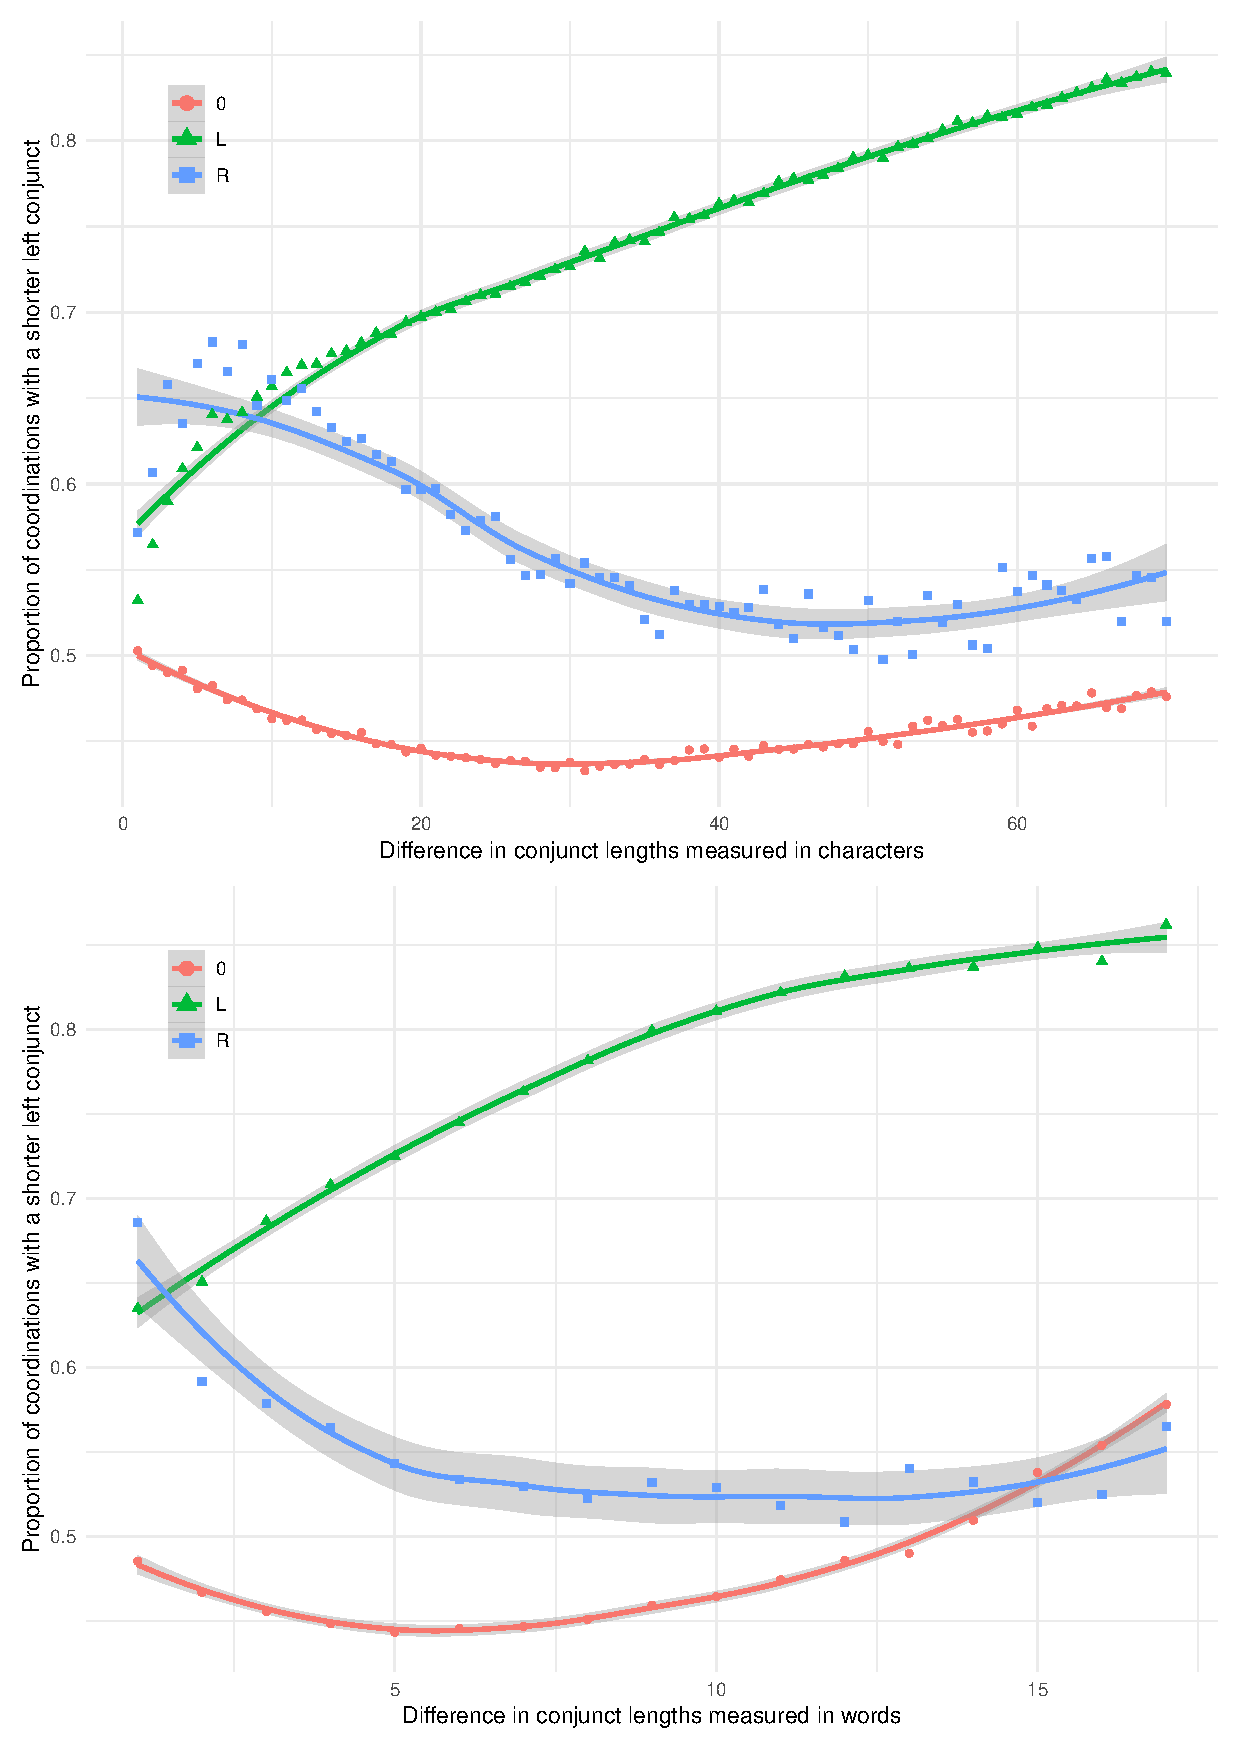
\includegraphics[width=\textwidth]{inputs/sud-observed.pdf}
    \caption{\centering Observed and loess-smoothed proportions of coordinations with shorter left conjuncts depending on the length difference between the conjuncts and on the position of the governor, data according to the SUD-trained model}\label{fig:sud-observed}
\end{figure}

\begin{figure}[hbt!]
    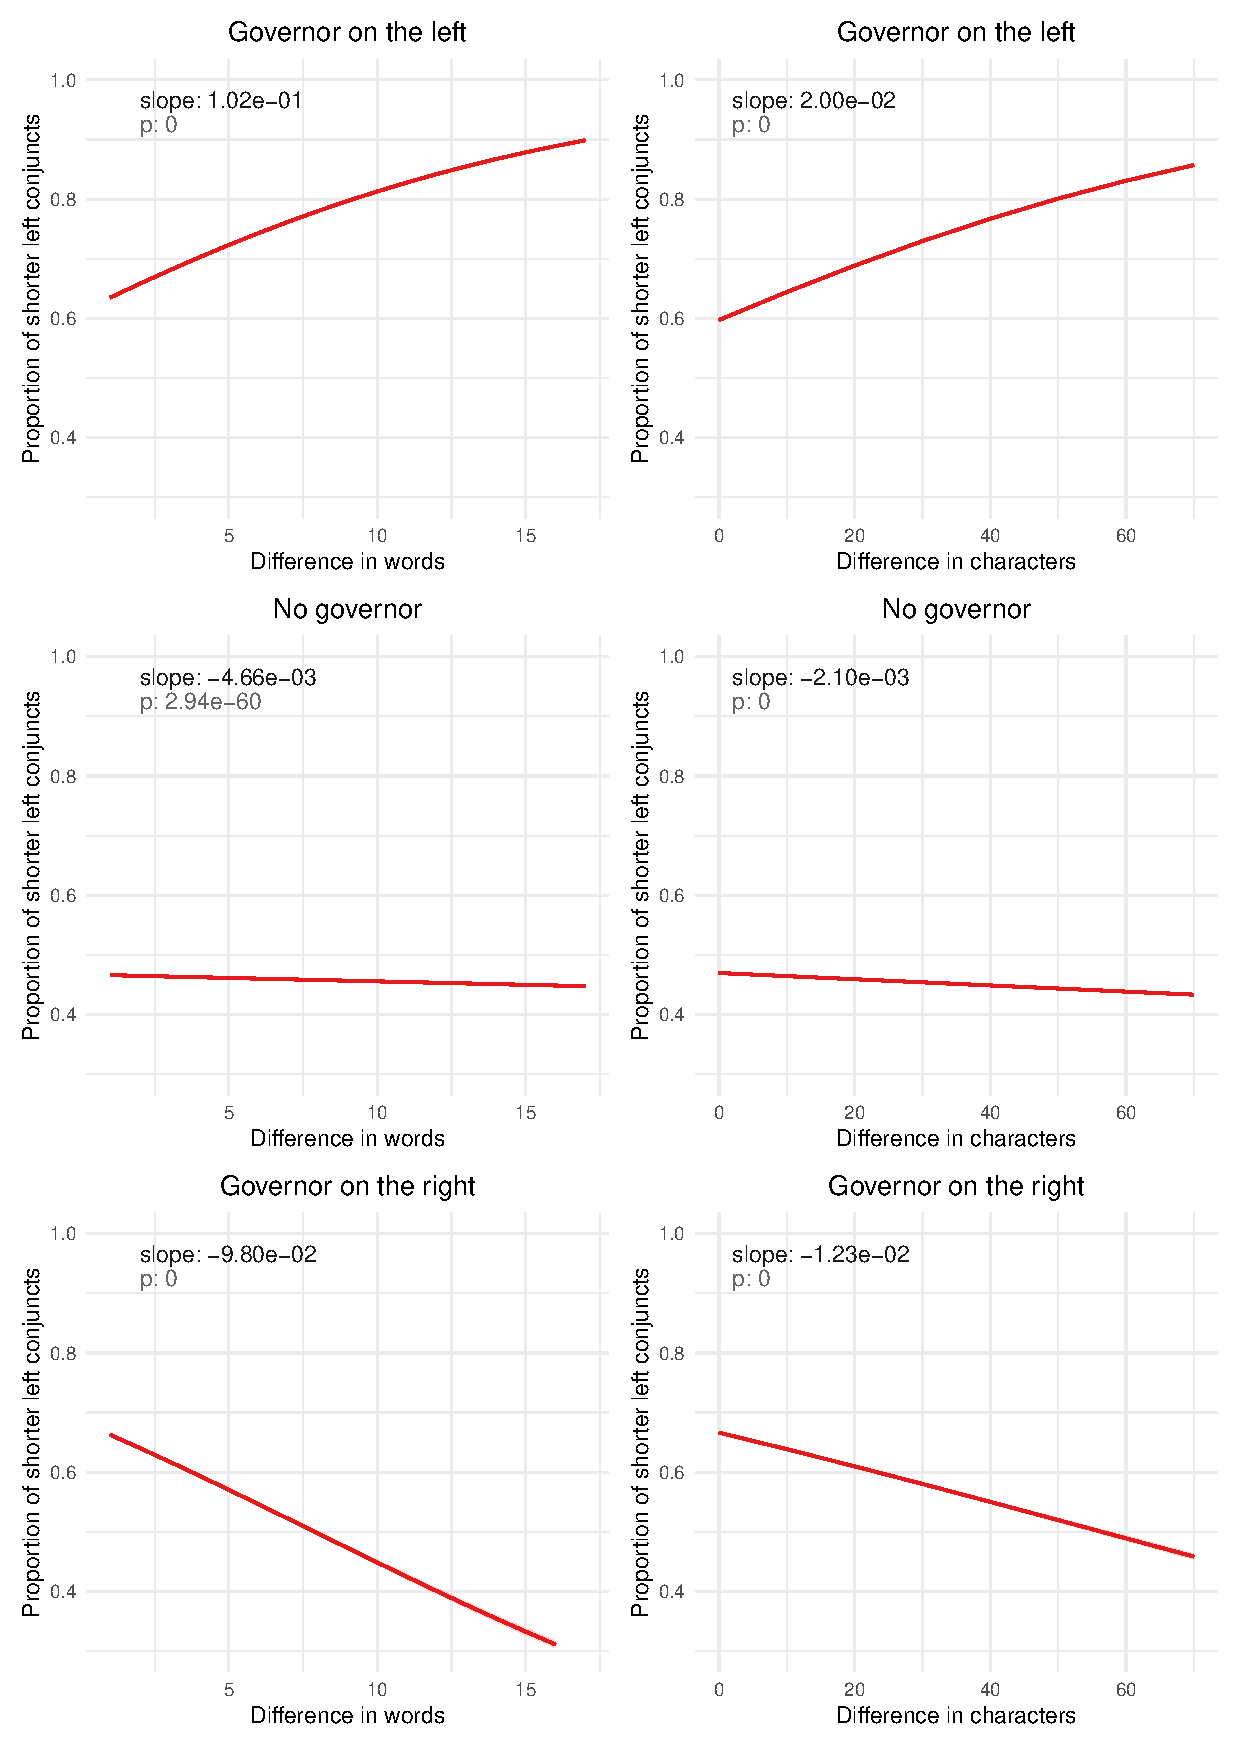
\includegraphics[width=\textwidth]{inputs/sud-modelled.pdf}
    \caption{\centering Modelled proportions of coordinations with shorter left conjunct depending on the length difference between the conjuncts, data according to the SUD-trained model}\label{fig:sud-logit}
\end{figure}

\begin{figure}[hbt!]
    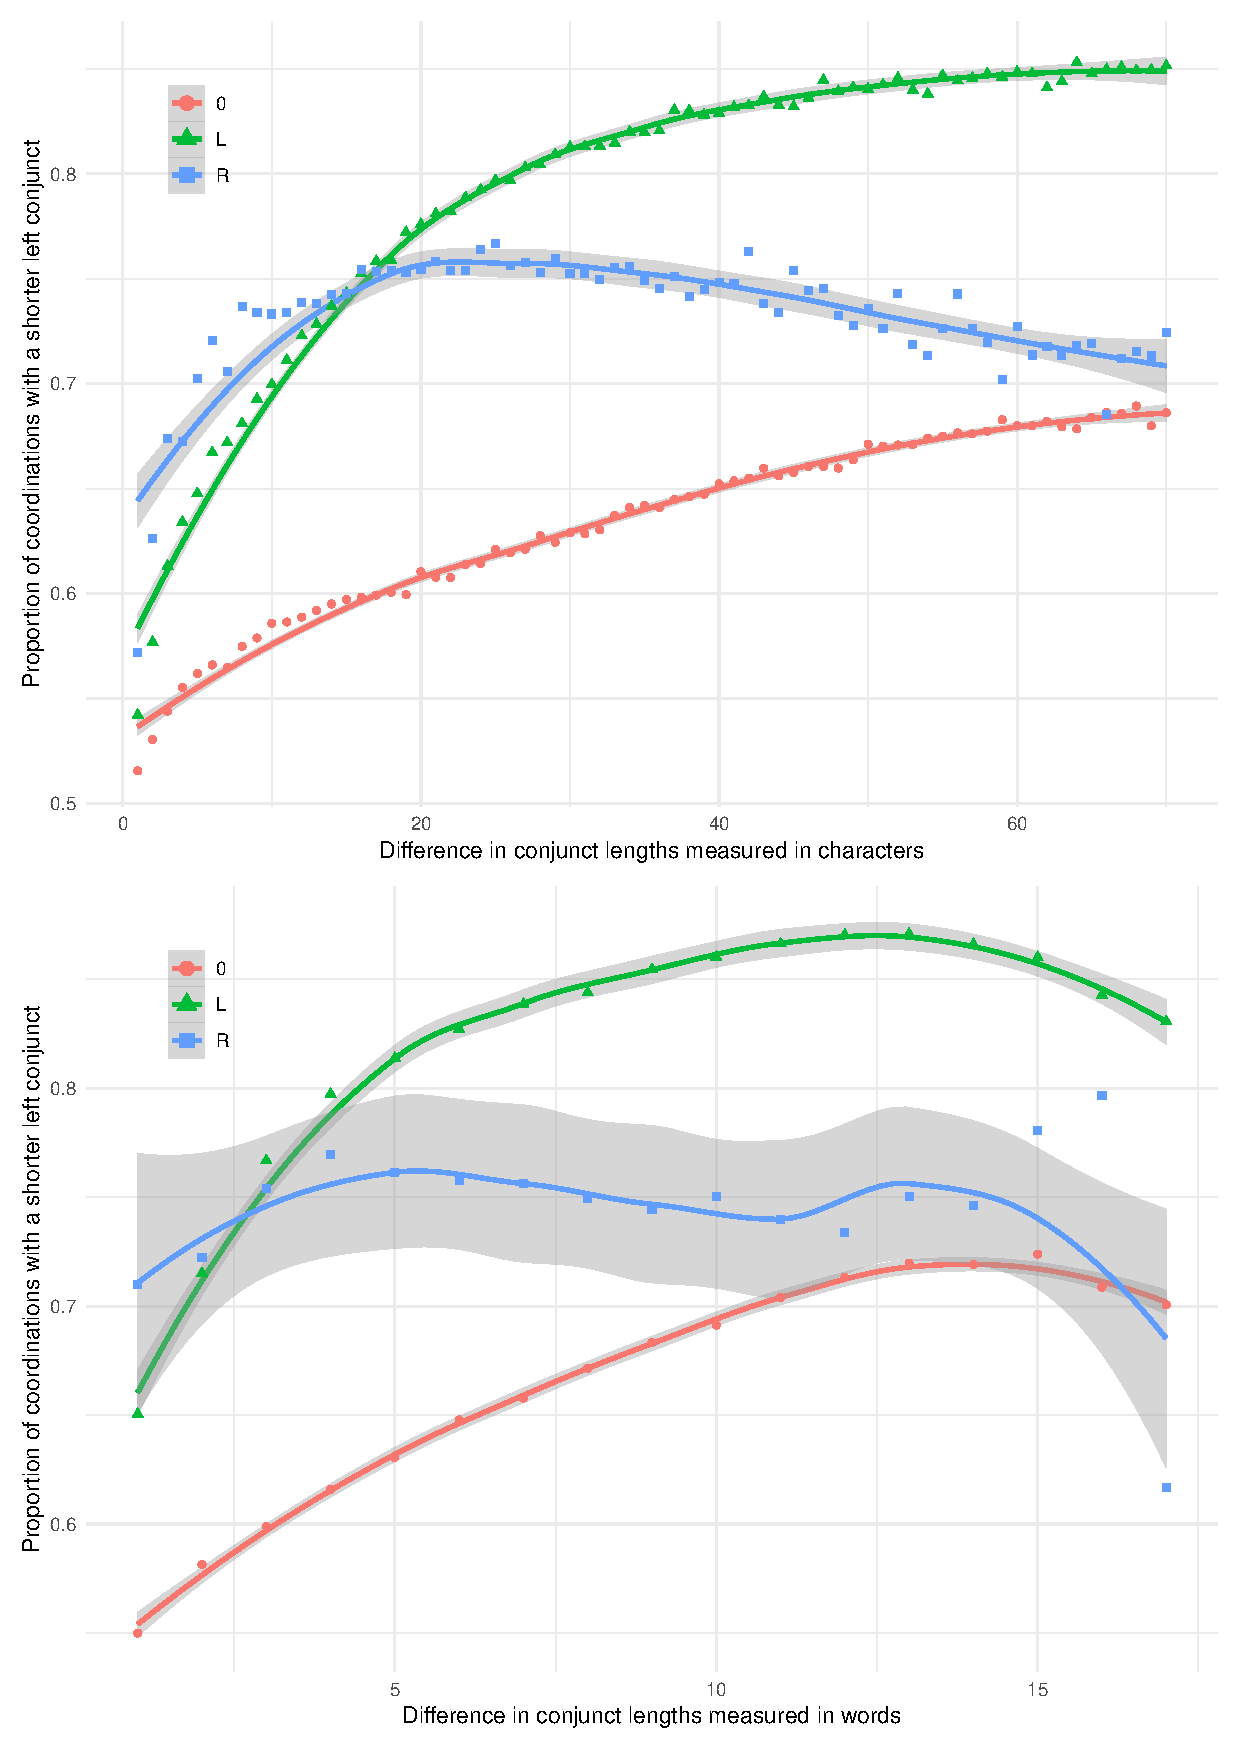
\includegraphics[width=\textwidth]{inputs/ud-observed.pdf}
    \caption{\centering Observed and loess-smoothed proportions of coordinations with shorter left conjuncts depending on the length difference between the conjuncts and on the position of the governor, data according to the UD-trained model}\label{fig:ud-observed}
\end{figure}

\begin{figure}[hbt!]
    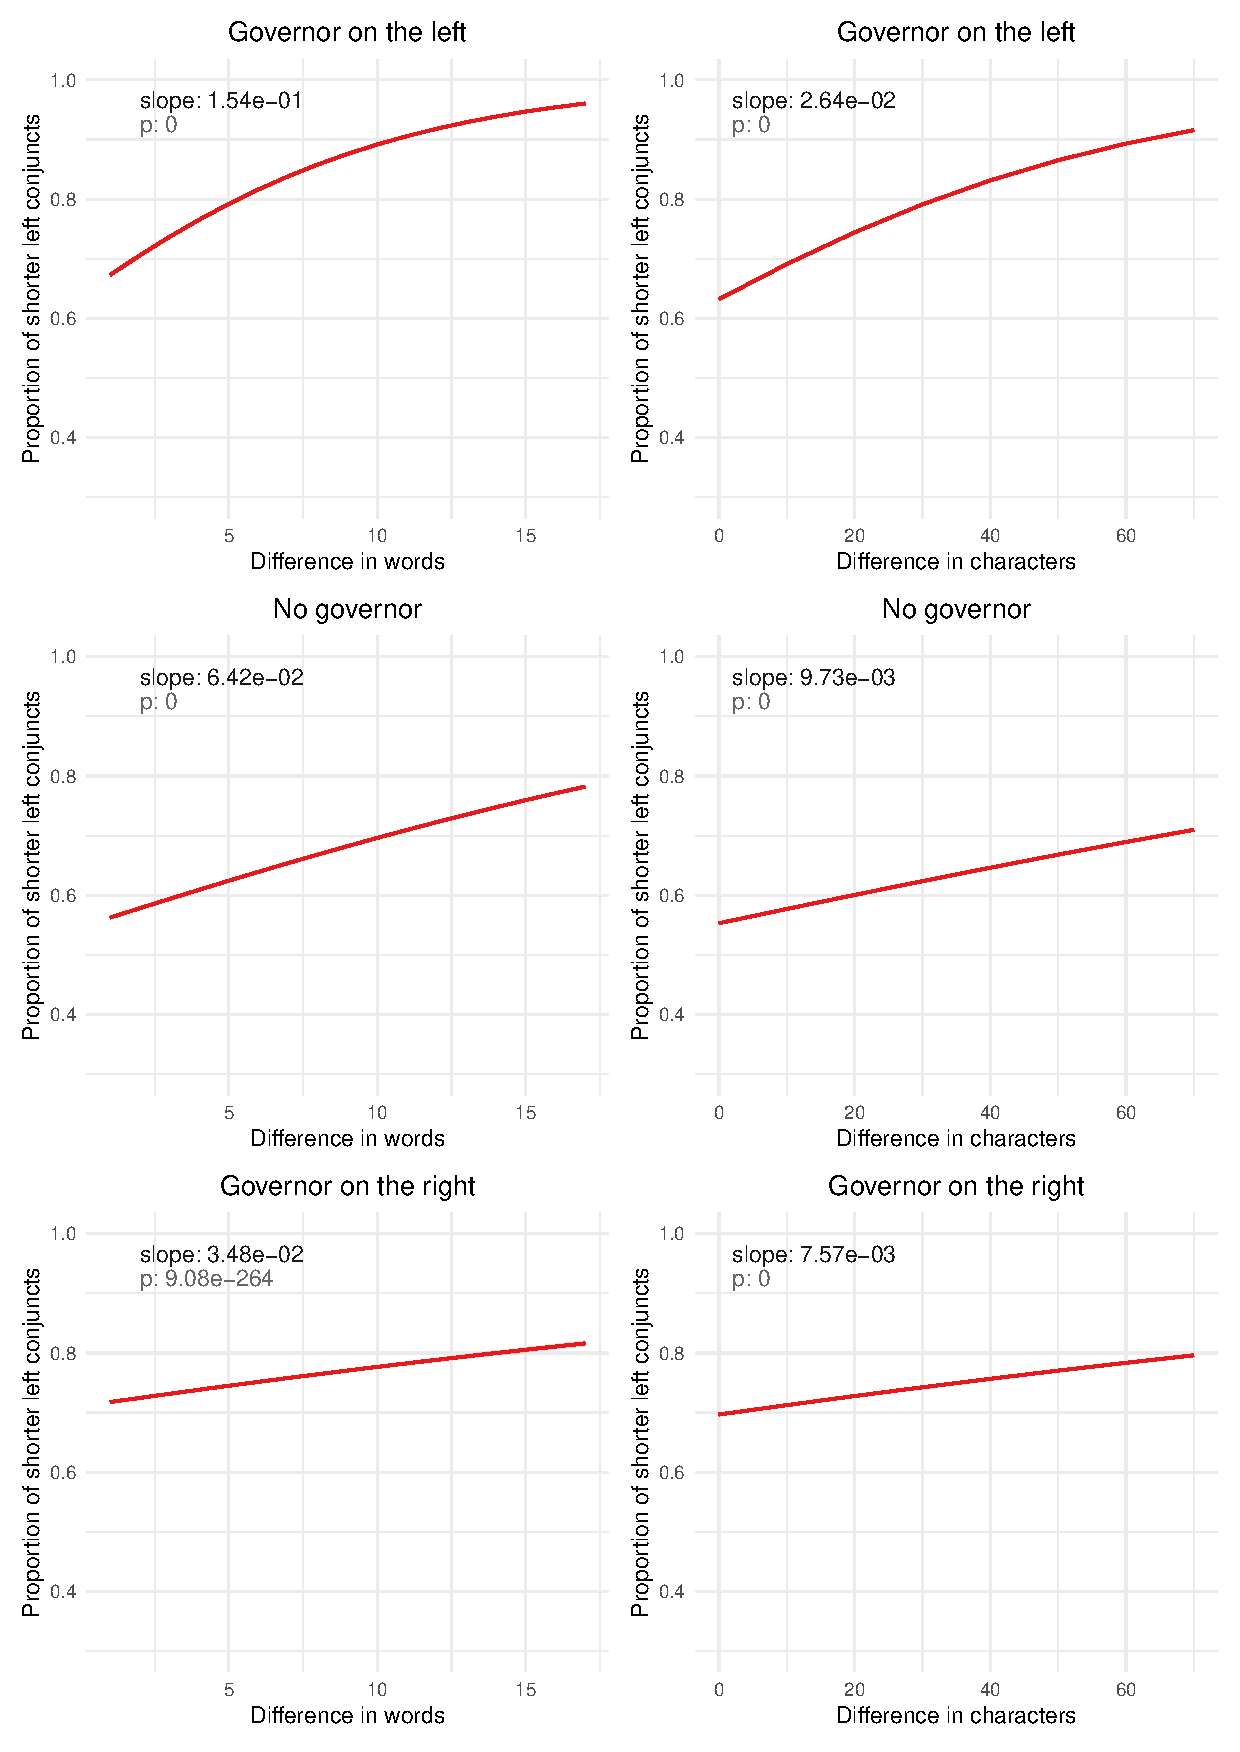
\includegraphics[width=\textwidth]{inputs/ud-modelled.pdf}
    \caption{\centering Modelled proportions of coordinations with shorter left conjunct depending on the length difference between the conjuncts, data according to the UD-trained model}\label{fig:ud-logit}
\end{figure}